\section{Task 2: approximation in inner-product spaces}
\subsection{Method overview and problem}
The task is to find the optimal approximation \( h^* \) of a function \( f \) in an inner-product space \( V \) by minimizing distance in a specified norm: \[
\|h^* - f\| = \inf \{\|u - f\| : u \in U\},
\] assuming \( U \) is a subspace of \( V \). Approximation-theory results imply:
\begin{itemize}
    \item The solution \( h^* \) exists and is unique.
    \item \( h^* \) is optimal if and only if \( f - h^* \) is orthogonal to \( U \), that is, \( \langle f - h^*, u \rangle = 0 \) for every \( u \in U \).
    \item \( h^* \) can be expressed as a linear combination of basis elements of \( U \).
\end{itemize}
\subsection{Solution method}
Assume the basis of \( U \) consists of functions \( \{f_i\}_{i \in I} \). Orthogonality of \( f - h^* \) to \( U \) gives: \[
\langle f - h^*, f_i \rangle = 0 \quad \text{for every } i \in I.
\] 
This gives a unique representation of \( h^* \):
\[
    h^* = \sum_{i \in I} a_i f_i.
\] 
The coefficients \( a_i \) of the approximation \( h^* \) in the basis of \( U \) can therefore be found by solving:
\[
\langle f, f_i \rangle = \sum_{j \in I} a_j \langle f_j, f_i \rangle.
\] 
in matrix form $Aa = b$:
\[
\begin{bmatrix} 
\left<f_1, f_1\right> & \left<f_2, f_1\right> & \cdots & \left<f_n, f_1\right> \\ 
\left<f_1, f_2\right> & \left<f_2, f_2\right> & \cdots & \left<f_n, f_2\right> \\ 
\vdots & \vdots & \ddots & \vdots \\ 
\left<f_1, f_n\right> & \left<f_2, f_n\right> & \cdots & \left<f_n, f_n\right> \\ 
\end{bmatrix} 
\begin{bmatrix} 
a_1 \\ a_2 \\ \vdots \\ a_n \\ 
\end{bmatrix} = 
\begin{bmatrix} 
\left<f, f_1\right> \\ 
\left<f, f_2\right> \\ 
\vdots \\ 
\left<f, f_n\right> \\ 
\end{bmatrix}
\]
\subsection{Tests} Approximation quality was evaluated as follows: \begin{itemize}
    \item Approximation errors were compared in the Chebyshev and $L^2$ metrics.
    \item Convergence to the original function was checked for different polynomial degrees.
\end{itemize} 
\begin{center}
\begin{minipage}{0.92\textwidth}
    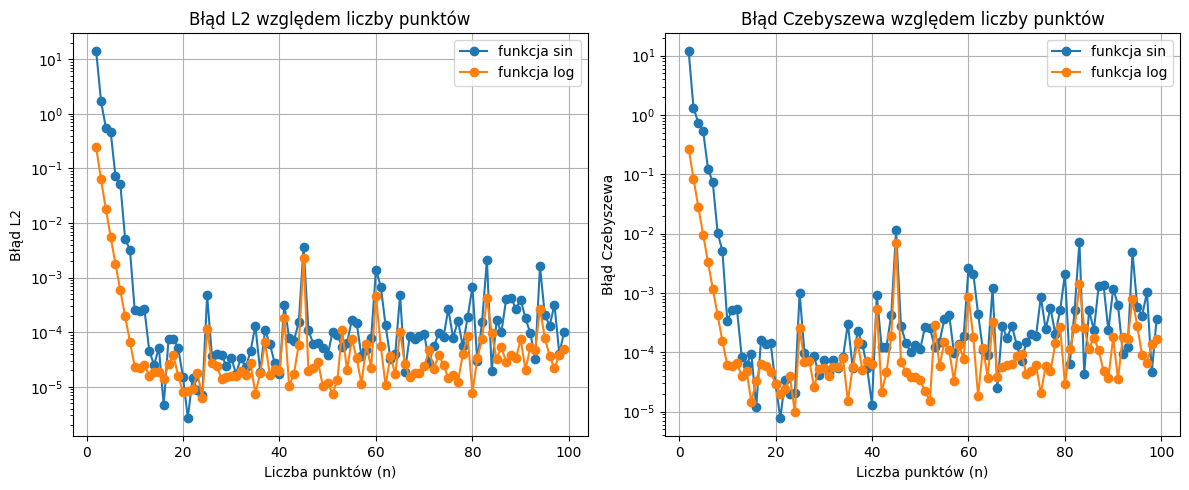
\includegraphics[width=\textwidth]{figures/task-2/error_points.png}
\end{minipage}
\hfill
\begin{minipage}{0.45\textwidth}
    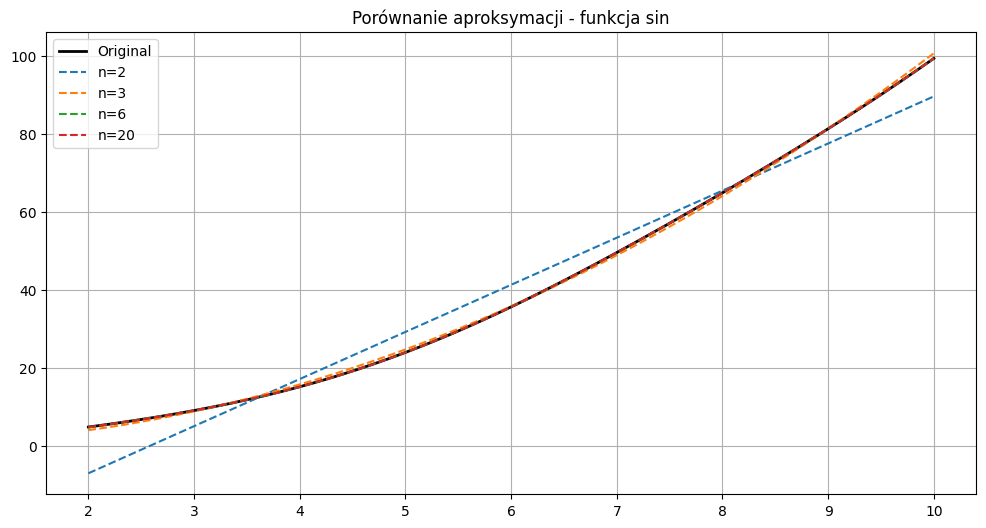
\includegraphics[width=\textwidth]{figures/task-2/comparison_sin.png}
\end{minipage}
\begin{minipage}{0.45\textwidth}
    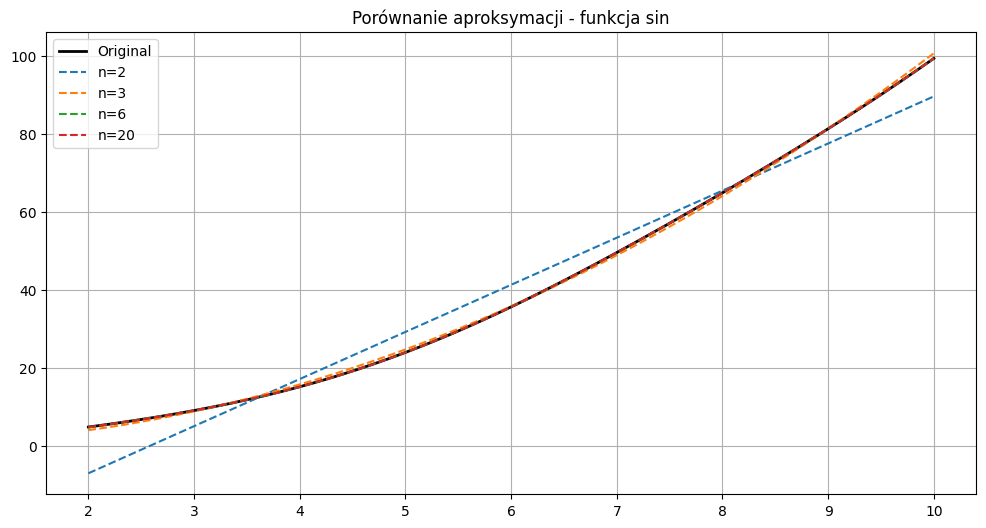
\includegraphics[width=\textwidth]{figures/task-2/comparison_sin.png}
\end{minipage}
\end{center}
\subsection{Conclusions and analysis}
\begin{itemize}
    \item Distance minimization with \( h^* \) gives smaller errors in both metrics than interpolation: previously $10^{-1}$, now $10^{-4} - 10^{-6}$.
    \item Functions approximated by \( h^* \) approach the original function faster, as the convergence plots show: previously around $25-30$, here $10-20$.
\end{itemize}
\paragraph{Computational-complexity comparison}
\begin{itemize}
    \item \textbf{Lagrange interpolation:} \( O(n^2) \).
    \item \textbf{Newton's method:} \( O(n^2) \).
    \item \textbf{Distance minimization \( h^* \):} \( O(n^3)\), because a linear system must be solved by the $LU$ method.
\end{itemize}
\paragraph{Conclusions}
\begin{itemize}
    \item Minimization with \( h^* \) gives better accuracy and faster convergence than the previous methods.
    \item Approximation accuracy increases exponentially with polynomial degree, allowing effective approximation even of functions with complex structure.
\end{itemize}
